\section{Evaluation on FPGAs}
\label{sec:exp}

% \zz{rename the section to Evaluation on FPGAs}
% \zz{we need to clearly state the purpose of this evaluation since we only implemented two simpler models; in addition to comparing with other xcels, it's important that we also evaluate the accuracy of our analytical model}

In this section, we implement two design points studied in \S\ref{sec:case_study} to validate the feasibility of our framework.
We first describe our experimental setup and perform evaluation on a single FPGA.

\subsection{Experiment Setup}
We test the publicly available BERT and GPT2 models listed in Table~\ref{tab:models}.
We conduct post-training quantization and use the W4A8 quantization scheme for BERT and the W8A8 scheme for GPT, which are prevalent settings in nowadays LLM inference~\cite{zhao2023atom,xiao2023smoothquant}.
% Non-linear layers remain using floating-point numbers. \yx{any reasons why we don't quantize non-linear layers?}
% The on-board results match the outputs from the quantized model in PyTorch and is able to achieve the same accuracy.
% \sout{Notice it is not the main focus of our paper, and all the quantization techniques should be orthogonal to our provided library.}
% Unless specially specified, we set the sequence length $l$ to $128$.

\begin{figure*}
    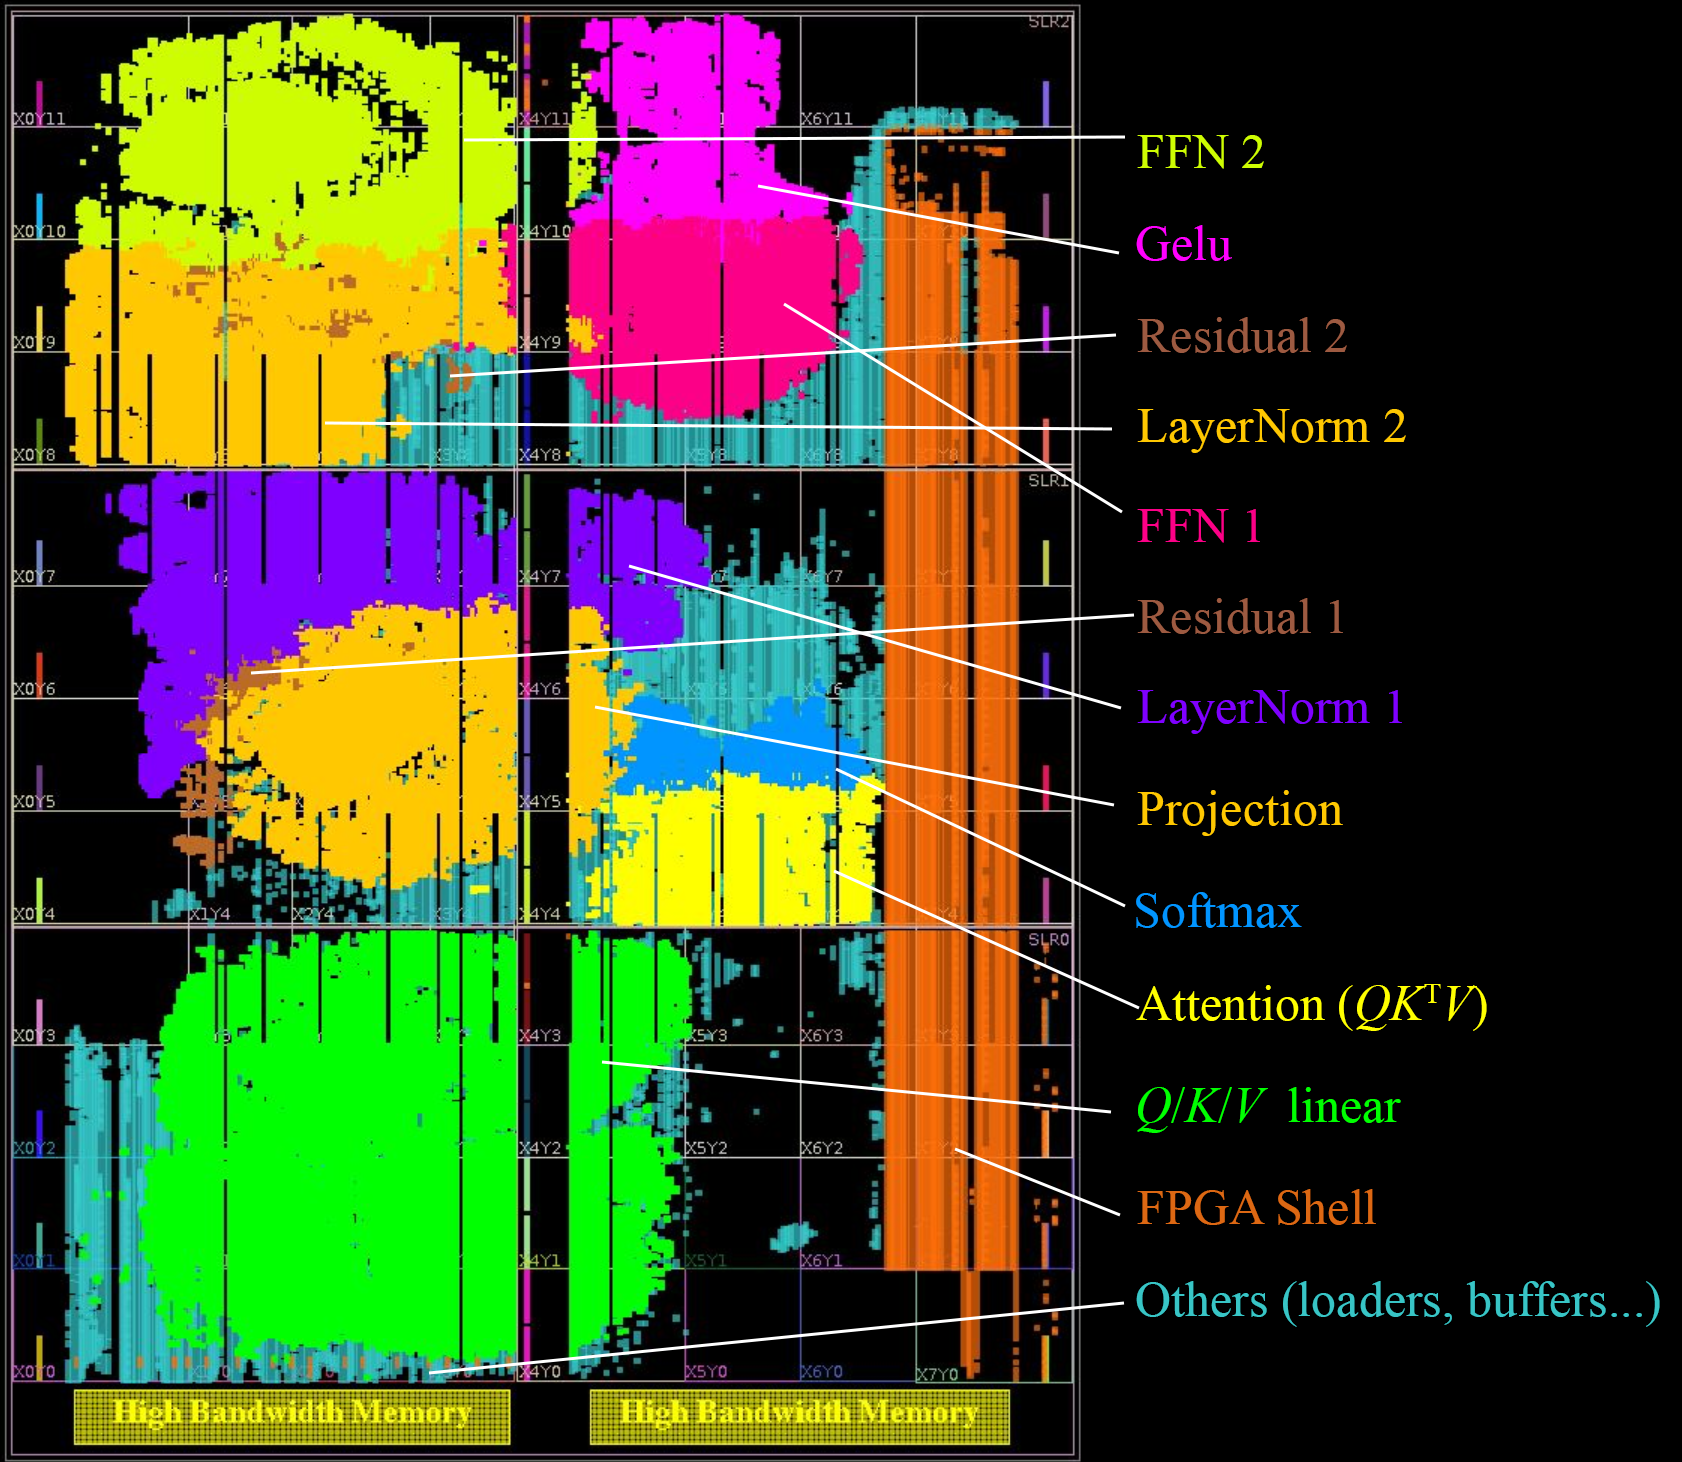
\includegraphics[width=0.5\linewidth]{figs/LLM.png}
    \caption{Physical layout of the implemented spatial accelerator.}
    \label{fig:device-layout}
\end{figure*}

We implement and run the actual design on an Alveo U280 FPGA~\cite{u280} with $M=256$ for the kernels.
This FPGA has 4032 BRAM18K blocks, 9024 DSP slices, 2.6M flip-flops, 1.3M LUTs, and 960 URAM blocks.
It has three SLRs with an almost equal amount of resources.
All the kernels are implemented in C++ with Vitis HLS v2022.1~\cite{vitis_hls_2022}, and synthesized with Vivado backend toolchains.
\revise{Figure \ref{fig:device-layout} shows the final device layout of the implemented accelerator.}
We use OpenCL with Xilinx RunTime (XRT) for hardware execution and Xilinx Board Utility (xbutil) for computing power measurements.
The environment for GPU experiments is listed in \S\ref{sub:workload_hardware}, and NVIDIA system management interface (nvidia-smi) is used for measuring GPU power.
Notice the quantized models on GPUs are slower than the FP16 models, as the quantization methods normally leverage fake quantization and lack high-performance GPU kernels to support efficient inference.
Therefore, we directly compare our accelerator with the best FP16 GPU results.
The FPGA on-board results match the outputs from the quantized model in PyTorch and are able to achieve the same accuracy.
The latency results are the average across fifty runs.

\subsection{On-Board Evaluation}
% 1. BERT latency (fixed seq_len) and area compared with other FQ-BERT[DATE'21] and FTrans[ISPLED'20]
% 2. GPT latency (variant seq_len) and energy efficiency compared with DFX[MICRO'21]

\begin{table*}
\centering
\caption{Experimental results compared with other FPGA-based accelerators. Sequence lengths are set as 512.}
\label{tab:bert_results}
\resizebox{\linewidth}{!}{
{
\begin{tabular}{l l l l l l l l l l l l}\Xhline{1pt}
\textbf{Name}  & \textbf{Device} & \makecell[l]{\textbf{Freq}\\\textbf{(MHz)}}  & \textbf{Quantization} &
% \begin{tabular}{c}
% \textbf{Latency (ms)}\\
% \textbf{\textcolor{gray}{(Est. \S\ref{subsubsec:latency})}}
% \end{tabular}
\makecell[l]{\textbf{Latency (ms)}\\\textcolor{gray}{[\textbf{Est. (\S\ref{sec:modeling})}]}}
& \makecell[l]{\textbf{Throughput}\\\textbf{(samples/sec)}} & \textbf{Speedup} & \textbf{BRAM} & \textbf{DSP} & \textbf{FF} & \textbf{LUT} & \textbf{URAM}\\
\Xhline{1pt}
\textbf{Ours} & U280 & 245 & W4A8 & 26.01 \textcolor{gray}{[24.07]} & \underline{\textbf{38.45}} & - & 389 (19\%) & 1780 (20\%) & 653K (25\%) & 569K (44\%)& 111 (12\%)\\
 - SLR0 & -& -& -& 4.86 & -& -& 130 (19\%) & 482 (17\%) & 200K (23\%) & 167K (38\%) & 3 (1\%)\\
 - SLR1 & -& -& -& 14.63 & -& -& 136 (20\%) & 590 (19\%) & 240K (28\%) & 212K (49\%) & 50 (16\%)\\
 - SLR2 & -& -& -& 19.81 & -& -& 123 (18\%) & 708 (23\%) & 213K (25\%) & 191K (44\%) & 58 (18\%)\\\hline
FQ-BERT~\cite{liu2021fqbert} & ZCU111 & 214 & W4A8 & 95.16 & 10.51 & \textbf{3.66$\times$} & 679 (31\%)& 3287 (77\%)& 201K (24\%)& 190K (45\%)& N/A\\\hline
TRAC~\cite{patrick2022trac} & ZCU106 & 200 & Fixed8 & 347.48 & 2.88 & \textbf{13.36$\times$} & 181 (29\%) & 1379 (80\%)& 128K (28\%)& 126K (55\%)& N/A\\
\Xhline{1pt}
\end{tabular}
}}
\end{table*}
\begin{figure*}
    \centering
    \includegraphics[width=\linewidth]{figs/exp/gpt2_results_est.pdf}
    \caption{Latency and energy efficiency of GPT2 model on different devices.
    The GPU results are obtained following the same setting in \S\ref{sec:case_study}.}
    \label{fig:gpt2_results}
\end{figure*}

We first compare our BERT accelerator with FQ-BERT~\cite{liu2021fqbert} and TRAC~\cite{patrick2022trac}, two FPGA-based accelerators for the BERT model.
To make a fair comparison, we employ the same W4A8 quantization precision with FQ-BERT and assess the model accuracy using the CoLA dataset~\cite{devlin2018bert}, a widely-used language understanding task.
The fp16 model achieves an accuracy of 56.84\%, while our W4A8 quantized model attains 56.76\% accuracy.
We only compare the performance of the core encoder layers, and \revise{report the best on-board latency results of the baselines obtained from the original papers.
Both baselines use a sequence length of 128, so we scale their latency results to match our sequence length of 512.
FTrans~\cite{li2020ftrans} also targets BERT-variant models, but it does not provide frequency and sequence length in the paper, so we cannot make a direct comparison.}
From Table~\ref{tab:bert_results},
% we can see that our accelerator is able to process the full sequence length (i.e., 512) as reported in the BERT paper~\cite{devlin2018bert}, while the other two accelerators can only process a reduced set of sequences.
we can see our spatial architecture delivers a much lower latency and a higher throughput with a much lower DSP usage.
Even though our evaluation device is not exactly the same as the baselines, our throughput improvement still surpasses the resource increment of FF and LUT.
Specifically, our accelerator is 3.66$\times$ faster than FQ-BERT~\cite{liu2021fqbert} and 13.36$\times$ faster than TRAC~\cite{patrick2022trac}.
% This is mainly due to the overlapped computation of different stages, memory and DSP packing, and higher frequency because of careful floorplanning.
\revise{Compared to temporal architectures, our spatial architecture can efficiently overlap the execution of the operators in the model and eliminate most of the data movement overhead.
In our design, one layer can start operation once the previous layer finishes computing one tile of the feature map, which typically takes only tens of cycles.
In contrast, temporal architectures need to wait for the entire tensor to be produced, which may take hundreds of cycles.
Therefore, even if the per-layer latency of spatial architectures is longer, the end-to-end latency can still be significantly lower than the temporal architectures employed by FQ-BERT and TRAC.}
Furthermore, our analytical framework precisely predicts the performance of the accelerator with less than 2ms of differences, showing the practicality of our approach.

We next design an accelerator for the GPT2 model.
We support importing quantized models from different quantization frameworks~\cite{xiao2023smoothquant,zhao2023atom,chee2023quip}.
Specifically, we export the W8A8 model from SmoothQuant~\cite{xiao2023smoothquant} and achieve 62.2\% on the LAMBADA dataset~\cite{denis2016lambada}, whereas the FP16 model demonstrates an accuracy of 65.0\%.
We compare our GPT accelerator with the state-of-the-art GPT accelerator, DFX~\cite{hong2022dfx}, which employs a temporal architecture with an instruction set and uses the same U280 FPGA device for on-board evaluation.
On average, we are 2.16$\times$ and 1.10$\times$ faster than DFX in the prefill and decode stage respectively.
This is because our spatial architecture overlaps the computation and greatly eliminates off-chip memory access.
% as much as possible.
% \zz{are we actually comparing power or energy efficiency? in the former case, we should say lower power not more efficient}
We can also see our estimations in \S\ref{sec:modeling} align closely with the actual performance, achieving a 92\% accuracy for the prefill stage.
For the decode stage, the estimated latencies are lower than the actual results, which is mainly because the initial interval between two operators is not significantly smaller than the execution time of one stage, contributing to a notable increase in latency.

We also include the GPU results in \S\ref{sec:case_study} for a more comprehensive evaluation.
As shown in Figure~\ref{fig:gpt2_results}, neither DFX nor our design performs well during the prefill stage compared to GPUs that have more compute resources to exploit the abundant parallelism.
Notably, the latency of FPGAs in the prefill stage increases linearly, while the GPU ones almost remain constant as the model does not fully utilize GPUs.
For the decode stage, the situation is reversed.
FPGA-based accelerators are more efficient than GPUs, and our accelerator can achieve a 1.85$\times$ speedup and is 5.69$\times$ more energy efficient compared to the A100 GPU.
This is because the generation of each token is fully sequential, and GPUs cannot leverage their abundant parallelism, and suffer from extensive memory access overheads.
On the contrary, our dataflow accelerator eliminates most of the off-chip memory accesses and overlaps the compute as much as possible.
Thus, we can achieve a better performance compared to GPUs, aligning with our estimation results in \S\ref{sec:case_study}.
Notice the U280 FPGA only uses a 16nm process while the A100 GPU has a more advanced 7nm process node based on the data in Table~\ref{tab:device}, but we can still achieve higher speedup, demonstrating the efficiency of our spatial accelerators.
It also indicates the potential of further optimizing our HLS design and scaling it up to achieve even higher performance.

\subsection{Ablation Study}
\label{sub:ablation}
% 1. Systolic array packed or not
% 2. Different stages latency breakdown
\revise{We begin by examining the latency of different SLRs.
As shown in rows 3-5 in Table~\ref{tab:bert_results}, the overall latency of the BERT accelerator is nearly the sum of the latency of SLR0 and SLR2, aligning with the pipeline diagram in Figure~\ref{fig:pipeline}.
Moreover, the computation in SLR1 largely overlaps with that of SLR2 due to the fully pipelined design.
The resource usage across different SLRs is also similar, resulting in a balanced design.}

We further investigate the efficiency of our kernel functions.
We conduct experiments on our template systolic array function with the AutoSA-generated systolic array, which is a highly optimized state-of-the-art systolic array implementation~\cite{wang2021autosa}.
From Table~\ref{tab:sa}, we can see our implementation achieves the same level of performance compared to AutoSA.
While maintaining the same DSP usage, the resource usage of our kernel function is much smaller than AutoSA.
\revise{Since the prediction of a single GEMM kernel is accurate and can achieve the theoretical performance, our analytical model can precisely predict the performance of spatial accelerators when combining multiple linear operators.}
The presence of latency-predictable kernels as foundational components plays a pivotal role in this predictability.
Additionally, our function offers enhanced customizability, accommodating varying sizes and the choice of different quantization schemes.

Moreover, employing DSP packing further reduces the DSP usage, allowing one DSP to handle two MAC operations within a single cycle, a feature not supported in AutoSA.
This experiment shows the efficiency of our kernels, facilitating the development of high-performance Transformer accelerators.
\begin{table}[!htbp]
\centering
\caption{Latency and resource usage of our systolic array library function. Results are directly derived from the HLS report in 300MHz.
The GEMM kernel is extracted from the first FFN layer in the BERT-base model with size $(512,768)\times(768,3072)$.
We use a 16~\X16 systolic array to calculate the \texttt{int8} GEMM.
The theoretical peak performance without DSP packing is $(512\times 768\times 3072)/(16\times 16)$ cycles $\times 3.33$ ns/cycle = $15.71$ ms.
}
\label{tab:sa}
\resizebox{\linewidth}{!}{
\begin{tabular}{ccccccc}\Xhline{1pt}
 & \textbf{Latency (ms)} & \textbf{Effective $M$} & \textbf{BRAM} & \textbf{DSP} & \textbf{FF} & \textbf{LUT}\\\Xhline{1pt}
Ours (w/o DSP packing) & 15.73 & 256 & 0 (0\%) & 256 (2\%) & 88284 (3\%) & 168190 (12\%)\\
Ours (w/ DSP packing) & 15.73 & 128 & 0 (0\%) & \textbf{128 (1\%)} &  79969 (3\%) & 244439 (18\%)\\
AutoSA~\cite{wang2021autosa} & 15.71 & N/A & 514 (12\%) & 256 (2\%) & 100138 (3\%) & 244032 (18\%)\\\Xhline{1pt}
\end{tabular}
}
\end{table}

\revise{Lastly, we analyze the performance of the non-linear operators.
As shown in Table~\ref{tab:nonlinear}, we observe that the softmax operator in the MHA module incurs the highest latency, primarily due to the need to compute the exponential function.
% Since there is no Gaussian cumulative distribution function on FPGA, we use a piecewise linear function to approximate the GeLU function.
Since these operators are elementwise and only require a row of data to start the computation, they can be easily fused with the preceding linear operators in the pipeline, thereby not significantly impacting the overall latency.
For instance, the combined latency of a GEMM kernel (10.77ms) and the softmax operator (6.67ms) greatly exceeds the latency of SLR1 in Table~\ref{tab:bert_results} (14.63ms$/$300MHz$\times$245MHz), indicating substantial overlap between the softmax operator and other operators.
Again, these ablation studies show that considering only the linear operators in the analytical framework is sufficient to achieve an accurate latency estimation.
}
\begin{table}[!htbp]
\centering
\caption{Performance and resource usage of non-linear operators in our kernel library.
Kernel sizes are set to match those of the BERT model in Table~\ref{tab:bert_results}.
Results are directly derived from the HLS report in 300MHz.}
\label{tab:nonlinear}
\small
{
\begin{tabular}{cccccc}\Xhline{1pt}
\textbf{Operator} & \textbf{Latency (ms)} & \textbf{BRAM} & \textbf{DSP} & \textbf{FF} & \textbf{LUT}\\\Xhline{1pt}
Softmax & 6.67 & 8 & 38 & 4835 & 7447\\
LayerNorm & 0.85 & 20 & 80 & 18751 & 12746\\
GeLU & 0.67 & 0 & 256 & 26193 & 16472\\\Xhline{1pt}
\end{tabular}
}
\end{table}

\begin{comment}
\subsection{Scaling Projection}
% 1. Communication cost (package size vs transmission time)
% 2. Extend to multiple FPGAs (latency compared to DFX)
We further project our experimental results to multiple FPGAs.
% Using multiple FPGAs brings more reconfigurable fabric and increased computing power, but it also introduces additional communication and synchronization overheads.
% These overheads may become the bottleneck and cancel out the expected speedup. 
\begin{figure}[t]
    \centering
    \includegraphics[width=0.7\linewidth]{figs/exp/projection.pdf}
    \caption{Scaling projection for multiple U280 FPGAs.}
    \label{fig:projection}
\end{figure}
To better model overheads in distributed inference, we base our analysis on a realistic multi-FPGA cluster from Open Cloud Testbed (OCT)~\cite{oct_fpga} which is equipped with 16$\times$ interconnected U280 FPGAs.
Each FPGA in the OCT cluster is connected to a shared 100 GbE Ethernet switch through two QSFP28 ports, and each QSFP28 port can provide up to 100 Gbps bandwidth for duplex communication~\cite{handagala2022octnetwork}.

We use the LLaMa-7B model in Table~\ref{tab:models} to study the performance implications of distributed inference on multiple U280 FPGAs in the OCT cluster.
Based on the GPT2 results in Figure~\ref{fig:gpt2_results} and \S\ref{sub:multifpga}, we can estimate the scaling results as shown in Figure~\ref{fig:projection}.
The actual effective bandwidth $\alpha B$ depends on various factors, such as network topology, congestion control, or routing policy.
To make our analysis more tolerant to sub-optimal network environments, we set $\alpha = 50\%$, which indicates the network bandwidth is underutilized~\cite{handagala2022octnetwork}.
From Equation~\eqref{eq:multilatency}, we can see that $T_{comm}$ only becomes a bottleneck when the TP size $p_1$ is large enough.
Suppose the sequence length is 512 and FP16 for activation.
For the prefill stage, the TP communication overhead for one all-reduce is $T_{\text{comm}}=ldb_A/(\alpha B) = 0.336ms$, while the scaled latency of one pipeline stage in Figure~\ref{fig:pipeline} for LLaMA is $227.46ms$, which is much larger than $T_{\text{comm}}$.
Thus, the communication can be hidden by computation based on Equation~\eqref{eq:multilatency}.
Similarly, for the decode stage, the TP communication overhead $T_{comm}=db_A/(\alpha B)=0.66\mu s$, while the latency of one pipeline stage is $0.65ms$.
Again, it is much larger than the communication time, so it will not be the bottleneck.
% Thus, we can conclude the communication overhead may only become the bottleneck when the TP group size is too high or when the network bandwidth is too low.

% As connecting multiple FPGAs together requires system privilege, we only measure the communication time between two U280 FPGAs.

%In our experiment, we use the AMD Xilinx XUP UDP stack and pre-built binary object files for the CMAC kernels to demonstrate sending and receiving UDP packets between two FPGAs. Our objective is to measure the round trip time between the two FPGAs. The sender node reads a specific number of packets from a text file and transmits them over the network layer and CMAC to the receiving node. On the receiver side, the incoming UDP packets are received as raw data. By measuring the time it takes for a packet to make the round trip, we can calculate the round trip time and assess the performance of the network.
% Table~\ref{tab:rtt} shows the results.


% \begin{table}[!htbp]
% \centering
% \caption{UDP/IP communication measurement between two FPGAs on the same rack.}
% \label{tab:rtt}
% \resizebox{\linewidth}{!}{
% \begin{tabular}{cccc}\Xhline{1pt}
% \textbf{Package Size (MB)} & \textbf{RTT ($\mu$s)} & \textbf{Throughput (GB/s)} & \textbf{\% of ideal} \\\Xhline{1pt}
% 0.001 & 270 & 0.07 & 0.52 \\
% 0.013 & 284 & 0.60 & 4.76 \\
% 0.134 & 450 & 1.25 & 9.99 \\
% 1.34 & 536 & 8.86 & 70.88 \\
% 26.86 & 6926 & 7.85 & 62.76\\\Xhline{1pt}
% \end{tabular}
% }
% \end{table}
\end{comment}